\documentclass[10pt,aspectratio=169]{beamer}
\usepackage{itmo/ITMOtheme}

\usepackage{pdflscape}		% pdfpages package requires the following packages
\usepackage{pdfpages}       %This package simplifies the insertion of external multi-page 
\usepackage{graphics}
\usepackage{subcaption}
\usepackage{array}

\usepackage{caption}
\captionsetup{skip=0.5pt}  % Set the space to 2 points

\usepackage[%
backend=biber, bibencoding=utf8,
sorting=none, style=gost-numeric,
%language=autobib,  autolang=other,
%clearlang=true,  defernumbers=true,
sortcites=true,
doi=false,
url=false, % add new: + doi, - url
isbn=false,
giveninits=true,
maxbibnames=99,
movenames=false, %Put the author's name first.
]{biblatex}
\addbibresource{papers.bib}

\hypersetup{
	unicode=true,
	colorlinks=true, % to remove []
	linkcolor = ITMOred,
	citecolor = ITMOgreen,
	urlcolor = ITMOblue,
}

%\setfootlinetext{Факультет систем управления и робототехники}
%\setfootlinetext{\insertsection}
%Thêm tùy chọn allowframebreaks vào môi trường frame để cho phép Beamer tự động chia nội dung thành nhiều frame khi cần thiết.
%\begin{frame}[allowframebreaks]{Frame with Long Content}


%Information author
\def\thesisname{Адаптивное управление системами с переменными параметрами}
\def\thesisauthor{Нго Данг Хиен}%, аспирант, 2-й год, факультет ФСУиР}
\def\supervisor{Герасимов Дмитрий Николаевич, доцент, к.т.н}%кандидат технических наук}
\def\speciality{2.3.1\par Системный анализ, управление и обработка информации, статистика}
%\dpartment{факультет систем управления и робототехники}
\def\email{hiennd@itmo.ru}
\def\where{Санкт-Петербург}
%\def\days{24 июня 2024}
\newcommand{\days}{\today}

%Tilte
\newcommand{\insertpagetitle}{
	\begin{frame}[plain,noframenumbering]
		\centering
		\itmopolygons{
			\begin{center}
				\vspace*{10pt}
				
\includegraphics[scale=0.1]{itmo/logo-basic-russian-white.pdf}
				\vfill
				
				{\bf \large \thesisauthor} \par
				\vspace*{10pt}
				
				{\bf \Large \thesisname} \par
				\vspace*{15pt}
				
				{Специальность: \speciality} \par
				\vspace*{15pt}
				
				{Научный руководитель: \par	\supervisor} \par
				
				\vfill
				\where, \days
				\vspace*{5pt}
			\end{center}
		}
	\end{frame}
}
%Outline
\newcommand{\insertoutline}{
	%\begin{frame}[label=toc]{Оглавление}%{План доклада}%{Outline}%[plain,noframenumbering]
		%\frametitle{Outline}
	%\begin{frame}[plain,noframenumbering]{Оглавление}
	\begin{frame}{Оглавление}
		\hypertarget{slide\insertframenumber}{}
		%\setbeamercolor{background canvas}{bg=blue}
		\large %\Large
		\tableofcontents
	\end{frame}
}
%Thanks
\newcommand{\insertpagethanks}{
	\begin{frame}[plain,noframenumbering]%{Вопросы?}
		\centering
		\itmopolygons{
			\begin{center}
				\vspace*{30pt}
				\begin{center}
					\textcolor{ITMOwhite}{\huge\textbf{Спасибо за внимание!}}
				\end{center}
				
				\vspace*{50pt}
				%			\begin{flushright}
					%				\textcolor{ITMOwhite}{E-mail: hiennd@itmo.ru}
					%			\end{flushright}
				\begin{exampleblock}{Контакты}
					\textcolor{ITMOwhite}{E-mail: \email}
				\end{exampleblock}
				\vspace*{10pt}
				\begin{figure}%[hb!]
					\centering
					
\includegraphics[scale=.1]{itmo/slogan-white.pdf}
			\end{figure}
		\end{center}
	}
	\end{frame}
}
%=====================================================================
\newcommand{\printPapers}{
	\begin{frame}{Публикации по теме работы} \hypertarget{slide\insertframenumber}{}
		\nocite{*}
		\printbibliography
	\end{frame}
}
\newcommand{\printConferenceRU}{
	\begin{frame}{Апробация работы} \hypertarget{slide\insertframenumber}{}
		\begin{enumerate}
			\item \textcolor{blue}{The 22nd IFAC World Congress}, Yokohama, Japan.  9–-14 июля 2023 г.
			\item \textcolor{blue}{The 63rd IEEE Conference on Decision and Control (CDC-2024)}, Milan, Italy. 16--19 декабря 2024 г.
			\item \textcolor{blue}{XIV Всероссийское совещание по проблемам управления (ВСПУ-2024)}, Россия, Москва, ИПУ РАН. 17--20 июня 2024 г.
		\end{enumerate}
		
	\end{frame}
}

	%modify user in here!
\newcommand{\redcolor}[1]{{\color{red} #1}}
\newcommand{\bluecolor}[1]{{\color{blue} #1}}



\def\begali#1{\begin{align}{#1}\end{align}}
\def\lab{\label}
\def\rea{\mathbb{R}}

\newtheorem{statement}{Утверждение}
\newtheorem{assumption}{Допущение}
%\newtheorem{assumption}{Предположение}

\usefonttheme{professionalfonts}


%%%%%%%%%%%%%%%%%%%%%%%%%%%%%%%%%%%%%%%%%%%%%%%%%%%%%%%%%%%%%%%%%
\begin{document}
%%%%%%%%%%%%%%%%%%%%%%%%%%%%%%%%%%%%%%%%%%%%%%%%%%%%%%%%%%%%%
	\insertpagetitle
	\insertoutline
	%%%%[slide 2]%%%%%%%%%%%%%%%%%%%%%%%%%%%%%%%%%%%%%%%%%%%%%%%%%%%%%%%%%%%%%	
	\section{Актуальность исследования}
	\setfootlinetext{Актуальность исследования}
	\begin{frame}{Актуальность}
	\hypertarget{slide\insertframenumber}{}	
	Современные технические системы наиболее точно могут быть описаны нестационарными математическими моделями, в которых параметры могут изменяться во времени.
	
	\vspace{5mm}
	
	\begin{figure}[!h]
		\begin{subfigure}[t]{0.3\textwidth}
			\centering
			%\includegraphics[width=0.83\linewidth]{images/AM.jpg}
			\includegraphics[width=0.5\linewidth]{example-image} 
			\caption{Модель асинхронного двигателя}
		\end{subfigure}
		\begin{subfigure}[t]{0.3\textwidth}
			\centering
			\includegraphics[width=0.8\textwidth]{example-image} 
			\caption{Системы позиционирования судна}
		\end{subfigure}
		\begin{subfigure}[t]{0.3\textwidth}
			\centering
			\includegraphics[width=0.8\textwidth]{example-image} 
			\caption{Модель динамики манипулятора}
		\end{subfigure}
		\vspace{2mm}
		\caption*{Примеры систем с переменными параметрами}
	\end{figure}
\end{frame}

\section*{Цель, задачи исследования}
\setfootlinetext{Цель, задачи исследования}
\begin{frame}{Цель, задачи} \hypertarget{slide\insertframenumber}{}	
	\textbf{Цель исследования.}
	Целью диссертационной работы является синтез законов адаптивного управления для класса нестационарных систем в условиях параметрической неопределенности постоянной матрицы состояния и переменной матрицы входов.
	
	\vspace*{2mm}
	\textbf{Задачи.}
	%Для достижения данной цели в рамках диссертации были поставлены и решены следующие задачи:
	\begin{enumerate}
		\item Синтез закона адаптивного управления по выходу для линейного нестационарного объекта, модель которого содержит переменные параметры, описываемые управляемым генератором с известной матрицей состояния.
		\vspace*{2mm}
		\item Синтез адаптивного наблюдателя производных выходной регулируемой переменной для нестационарного объекта с параметрически неопределенной моделью переменных элементов матрицы входа.
		\vspace*{2mm}
		\item Синтез алгоритма адаптивного управления по выходу для класса нестационарных систем в условиях параметрической неопределенности с приложением для асинхронного двигателя с неизвестными сопротивлением, индуктивностью и моментом нагрузки.
	\end{enumerate}
\end{frame}
	
	\section{Обзор существующих методов}
	\setfootlinetext{Обзор существующих методов}
	\begin{frame}{Обзор существующих методов} \hypertarget{slide\insertframenumber}{}
	%	\scriptsize
	\begin{tabular}{|m{10cm}|m{4.4cm}|}
		%		\hline
		%	& Матрица состояния генератора \\
		\hline
		Ortega R., Loria A., Nicklasson P. J., Sira-Ramirez H. Generalized AC
		motor // Passivity-based Control of Euler-Lagrange Systems: Mechanical,
		Electrical and Electromechanical Applications. — London : Springer London,
		1998. — С. 265—309. & Параметрическая \redcolor{определенность} модели, Матрица входов -- \redcolor{обратная функция} \\
		\hline
		Данг Б. [др]. Метод синтеза адаптивных наблюдателей для нестационарных систем с полиномиальными параметрами [10.2021] &	Собственные числа матрицы состояния генератора параметров \redcolor{известны} и \redcolor{все равны 0}  \\
		\hline
		Низовцев С.И., Адаптивные наблюдатели линейных нестационарных систем в условиях неизмеряемых возмущений [12.2021] 
		
		Pyrkin A., Bobtsov A., Ortega R., Isidori A. An adaptive observer for uncertain linear time-varying systems with unknown additive perturbations//Automatica, 2023, Vol. 147, pp. 110677 & Собственные числа матрицы состояния генератора параметров  могут иметь \bluecolor{произвольные} значения, но \redcolor{известны} \\
		\hline
		Gerasimov D., Popov A., Hien N.D., Nikiforov V. Adaptive control of LTV systems with uncertain periodic coefficients //IFAC-PapersOnLine, 2023, Vol. 56, No. 2, pp. 9185-9190 & Матрица состояния \bluecolor{переменная}, матрица входов \redcolor{постоянная},  \redcolor{доступен измерению \par вектор состояния } \\
		\hline
		Нгуен Х.Т. Адаптивное оценивание нестационарных параметров с использованием метода внутренней модели [06.2023] & Собственные числа могут иметь \bluecolor{произвольные} значения и \bluecolor{неизвестны}, но для \par \redcolor{дискретной} модели \\
		\hline
		
	\end{tabular}
\end{frame}

%\section*{Научная новизна}
\begin{frame}{Научная новизна} \hypertarget{slide\insertframenumber}{}
	\textbf{Научная новизна} 
	\vspace*{0.5cm}
	\begin{itemize}
		\item 	 Разработка новых алгоритмов управления по выходу для класса нестационарных моделей на основе адаптивного наблюдателя переменных параметров, описываемых автономным или управляемым генератором с неизвестными начальными условиями и матрицей состояния.
		\vspace*{2mm}
		\item  Разработка нового метода параметризации модели генератора к виду линейного регрессионного соотношения, в котором вектор неизвестных параметров соответствует параметрам генератора.
		\vspace*{2mm}
		\item  Синтез закона управления по выходу для нестационарного объекта с неизвестными параметрами, предполагающий включение в контур управления цепочки интеграторов и гарантирующий асимптотическую устойчивость замкнутой системы.
	\end{itemize}
\end{frame}


\begin{frame}{Обобщенная постановка задачи}	\hypertarget{slide\insertframenumber}{}
	Рассматривается неафинный по входу объект управления
	\begin{align}
		\label{plant_x}
		\dot x(t) &= \redcolor{A}x(t) + \redcolor{B(t)} u(t),\\
		\label{plant_y}
		y(t) &= Cx(t),
	\end{align}
	где  $x(t)\in\rea^k$ ---  вектор переменных состояния,  $y\left( t \right) \in \rea{^m}$ --- измеримый вектор выходных регулируемых переменных,  $u\left( t \right) \in\rea {^\ell}$ ---   управляющих воздействий, элементы матрицы $A$ могут быть неизвестны, $B(\xi(t),u): \rea^{k\times\ell}$ --- матрица входов с переменными и неизвестными параметрами, $\xi(t) \in \rea^n$ --- вектор переменных состояния входной динамики, описываемой соотношением
	\begin{align}
		\label{Bxiu}
		\redcolor{B(t)} &= B_0\,H(\xi(t)),\\
		\label{xi}
		\dot{\xi}(t) &=\redcolor{\Gamma}\xi(t) +Gu(t),
	\end{align}
	где элементы матрицы $\Gamma$ могут быть неизвестны, $B_0\in\rea^{k\times r}$ --- известная матрица, $H(\xi(t)): \rea^n \to \rea^{r\times \ell}$
\end{frame}

\begin{frame} \hypertarget{slide\insertframenumber}{}
	Желаемое поведение выходной переменной $y^*(t)$ задано в виде выхода линейного генератора с состоянием $\xi_y(t)\in \rea^q$ и заданными параметрами $h_y\in\rea^{q\times m}$, $\Gamma_y \in\rea^{q\times q}$, $\xi_y(0)\in \rea^q$:
	\begin{align}\label{xi_star}
		\dot \xi_y(t)&=\Gamma_y\xi_y(t),\\
		\label{y_star}
		y^*(t)&=h_y^\top\xi_y(t).
	\end{align}
	
	Требуется синтезировать закон управления $u(t)$ по выходу,
	гарантирующий ограниченность всех переменных состояния, а также асимптотическое слежение регулируемой переменной $y(t)$ за задающим воздействием $y^*$:
	\begin{align}
		\label{goal}
		\mathop {\lim }\limits_{t \to \infty } \left( {A  - \hat A(t)} \right) = 0, \;
		\mathop {\lim }\limits_{t \to \infty } \left( {B(t)  - \hat B(t)} \right) = 0, \;
		\mathop {\lim }\limits_{t \to \infty } \left( {y(t)  - y^*(t)} \right) = 0.
	\end{align}
\end{frame}


\begin{frame} \hypertarget{slide\insertframenumber}{}
	%\small
	\begin{assumption}
		\label{ass1}
		Функция $B(t)$ такая, что матрица $B_0$ известна, пара $(A,B_0)$ является полностью управляемой, а также существует псевдообратное отображение $H^L(\xi,\tau):\rea^n\times\rea^r\to\rea^\ell$, удовлетворяющее соотношению
		\[	H\left(\xi\right)H^L(\xi,\tau)=\tau \]	
		для некоторой переменной $\tau\in\rea^r$ и $\forall\xi$.
	\end{assumption}
	\begin{assumption}
		\label{ass2}
		Пара матриц $(A, C)$ является полностью наблюдаемой.
	\end{assumption}
\end{frame}
	
	%%%%[Задача 1]%%%%%%%%%%%%%%%%%%%%%%%%%%%%%%%%%%%%%%%%%%%%%%%%%%%%%%%%%%%%%
	\section{Задача 1}
	\setfootlinetext{Задача 1}
	\begin{frame} \hypertarget{slide\insertframenumber}{}
	\centering
	\LARGE Задача 1: Синтез закона адаптивного управления по выходу для линейного нестационарного объекта с управляемым генератором переменных параметров с известной матрицей состояния.
	\end{frame}
	%================================
	\begin{frame}{Постановка задачи} \hypertarget{slide\insertframenumber}{}
	Рассматривается объект управления
	\begin{align}
		\label{8}
		\dot x(t) &= Ax(t) + B(t)\redcolor{u(t)},\\
		\label{9}
		y(t) &= C^\top x(t),
	\end{align}
	где  $x(t)\in\rea^k$,  $y\left( t \right) \in \rea^m$,  $u\left( t \right) \in\rea^\ell $, \par 
	\vspace{4mm}
	$B(t)=B(\xi(t))$ --- матрица входов с переменными параметрами
	\begin{align}	\label{10}
		B(t) &= B_0 \,  \xi^\top (t) H,\\
		\label{11}
		\dot \xi(t) &=\Gamma \xi(t)+G\redcolor{u(t)},
	\end{align}
	где $\xi(t) \in \rea^n$, \redcolor{$\xi(0)$} --- неизвестны, матрицы $ \Gamma, G$, $ B_0 \in \rea^k$, $H\in\rea^{n \times \ell}$ --- известны.
	
	\vspace{4mm}
	
	Требуется синтезировать закон управления $u(t)$, обеспечивающий ограниченность всех переменных состояния и выполнение целевого условия
	\begin{align}\label{12}
		\mathop {\lim }\limits_{t \to \infty } \left( {y(t)  - y^*(t)} \right) = 0.
	\end{align}
	
\end{frame}

\begin{frame}\frametitle{Синтез закона управления по выходу}
	\small %\scriptsize %\footnotesize %
	\begin{statement} \label{st2}
		Закон управления вида 
		\begin{align}\label{16}
			u(t) &= H^\top \xi_d V(t) +K_1^\top \redcolor{\xi(t)}, \\ 
			\dot \xi_d(t) &= (\Gamma +GK_1^\top)\xi_d(t) + GH^\top \xi_d(t)V(t), \\  
			V(t) &=  (\xi_d^\top(t) HH^\top \xi_d(t))^{-1} (\bluecolor{\tau(t)} - \xi_d^\top(t) HK_1^\top \xi_d(t)),
		\end{align}
		где начальные условия  $\xi_d(0)$ выбраны так, что $\|\xi_d(t)\|\in {\cal L}_\infty$ и $H^\top \xi_d(t) \neq 0$, с входным сигналом
		\begin{align}
			\bluecolor{\tau(t)} &= K_2^ \top \left( {\hat x\left( t \right) - {x^*}\left( t \right)} \right) + h_y^ \top \Gamma _y^k{\xi _y}\left( t \right),\\  \label{20}
			\dot{\hat x}\left( t \right) &= A\hat x\left( t \right) + B_0 \tau \left( t \right) + L\left(y(t) - C^\top \hat x(t)\right),
		\end{align}
		где	${x^*}\left( t \right) = \left[ {\begin{array}{*{20}{c}}
				{h_y^ \top } \\ 
				\vdots  \\ 
				{h_y^ \top \Gamma _y^{k - 1}} 
		\end{array}} \right]{\xi _y}\left( t \right)$, обеспечивает ограниченность всех переменных состояния и выполнение цели 
	\end{statement}	
\end{frame}


\begin{frame}{Оценка переменной $\xi(t)$}
	\hypertarget{slide\insertframenumber}{}
	%\small
	Продифференцируем \eqref{9} $k$ раз, перепишем в матричном виде, выразим вектор переменных $x(t)$ и подставим в уравнение $y^{(k)}(t)$. 
	\begin{align}\label{22}
		y^{(k)}= C^\top A^k \, W_y^{-1} \left( \varphi - F_1(u)\bluecolor{\xi} -F_2(u) \right) + C^\top A^{k-1}B_0 u^\top H^\top \bluecolor{\xi} + \ldots + {C^\top}{B_0}{\left( {\frac{d}{{dt}}} \right)^{k-2}}\left[ u^\top H^\top Gu \right].
	\end{align}
	
	Для исключения в выражении \eqref{22} неизмеряемой функции $\xi(t)$ воспользуемся методом GPEBO и рассмотрим фильтры вида
	\begin{align} \label{2.sigma1.ru}
		\dot \sigma_1 &= \Gamma \sigma_1 + Gu, \; \sigma_1(0)=0, \\
		\label{2.sigma2.ru}
		\dot \sigma_2 &= \Gamma \sigma_2, \qquad \sigma_2(0) =I.
	\end{align}
	Заметим, что для невязки $\tilde \xi(t) = \xi(t) - \sigma_1(t)$ имеем соотношение
	\begin{align*}
		\dot {\tilde {\xi}}(t)  = \Gamma \tilde \xi(t), \qquad
		\tilde \xi(0) =\xi(0),
	\end{align*}
	и $\tilde \xi(t)= \sigma_2(t)\xi(0)$. 
\end{frame}


\begin{frame}{Пример численного моделирования  1} \hypertarget{slide\insertframenumber}{}
	\begin{figure}[!h]
		\begin{subfigure}[t]{0.45\textwidth}
			\centering
			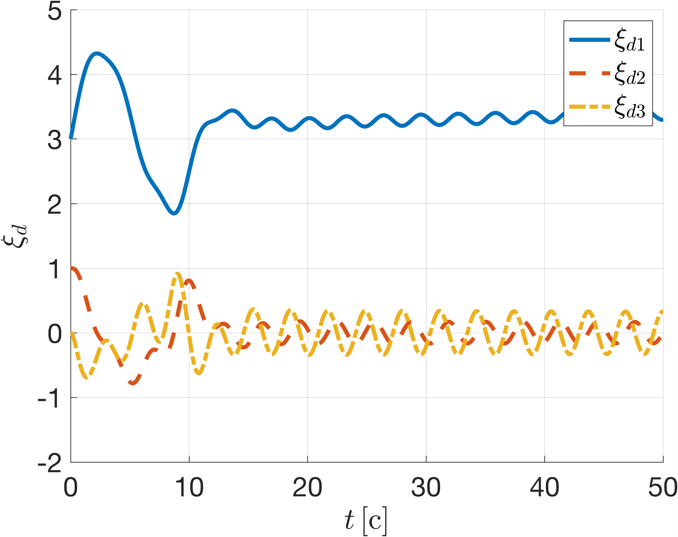
\includegraphics[width=0.5\linewidth]{figures/3.1xid.png}
			\caption{Временная диаграмма  $\xi_d$.}
		\end{subfigure}
		\begin{subfigure}[t]{0.45\textwidth}
			\centering
			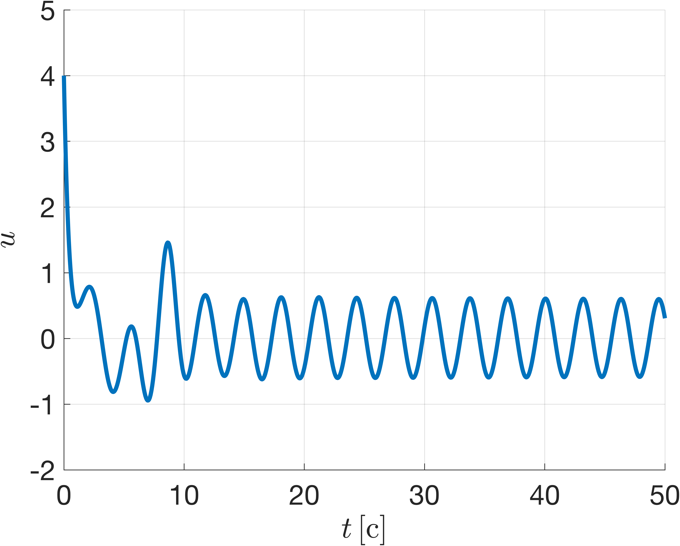
\includegraphics[width=0.5\linewidth]{figures/3.1u.png}
			\caption{Сигнал управления $u(t)$.}
		\end{subfigure}
		\begin{subfigure}[t]{0.45\textwidth}
			\centering
			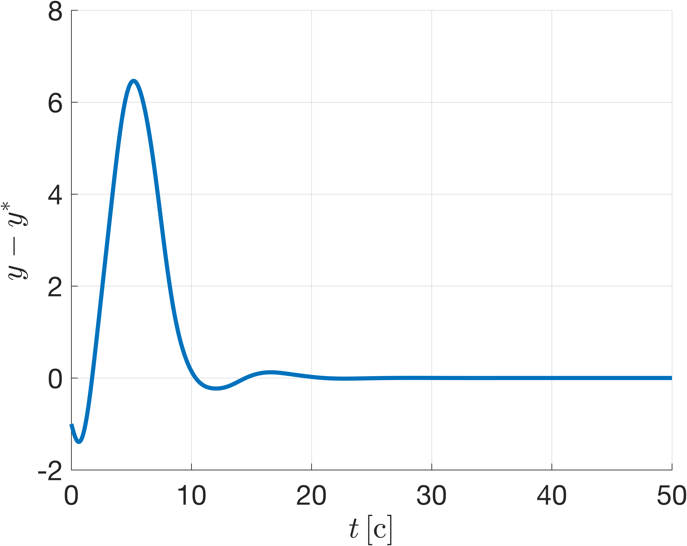
\includegraphics[width=0.5\linewidth]{figures/3.1ey.png}
			\caption{Ошибка регулирования $e(t)=y-y^*$.}
		\end{subfigure}
		\begin{subfigure}[t]{0.45\textwidth}
			\centering
			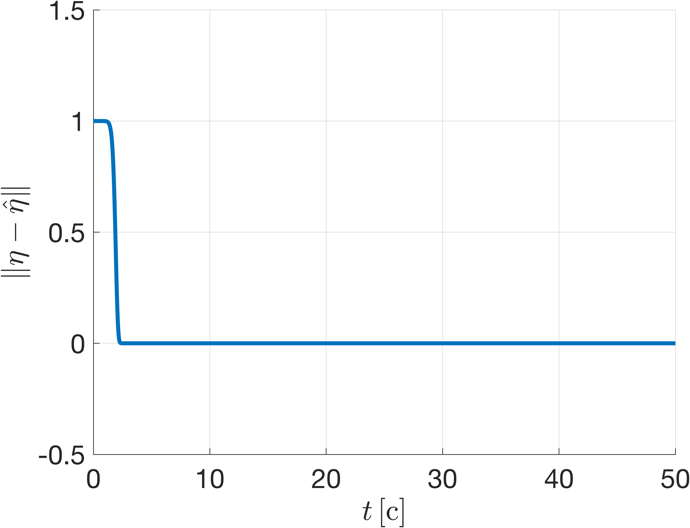
\includegraphics[width=0.5\linewidth]{figures/3.1eeta.png}
			\caption{Ошибка оценивания $\eta = \tilde \xi(0)$.}
		\end{subfigure}
		\label{f1}
	\end{figure}
\end{frame}
	%%%%[Задача 2]%%%%%%%%%%%%%%%%%%%%%%%%%%%%%%%%%%%%%%%%%%%%%%%%%%%%%%%%%%%%%
	\section{Задача 2}
	\setfootlinetext{Задача 2}
	\begin{frame} \hypertarget{slide\insertframenumber}{}
	\centering
	\LARGE Задача 2: 
	\end{frame}
	%================================
	\input{sections/section4.tex}
	%%%%[Задача 3]%%%%%%%%%%%%%%%%%%%%%%%%%%%%%%%%%%%%%%%%%%%%%%%%%%%%%%%%%%%%%
	\section{Задача 3}
	\setfootlinetext{Задача 3}
	\begin{frame} \hypertarget{slide\insertframenumber}{}
		\centering
		\LARGE Задача 3: 
	\end{frame}
	%================================
	\input{sections/section5.tex}
	%%%%[Задача 4]%%%%%%%%%%%%%%%%%%%%%%%%%%%%%%%%%%%%%%%%%%%%%%%%%%%%%%%%%%%%%
	
	%%%%[Заключение]%%%%%%%%%%%%%%%%%%%%%%%%%%%%%%%%%%%%%%%%%%%%%%%%%%%%%%%%%%%%%
	\section{Заключение}
	\setfootlinetext{Заключение}
	\begin{frame}{Заключение}
	%\begin{frame}{Положения, выносимые на защиту.}
		\hypertarget{slide\insertframenumber}{}
		\begin{itemize}
			\item Алгоритм управления по выходу для нестационарного объекта с переменной матрицей входа, параметры которой являются выходом управляемого генератора с известной матрицей состояния.
			\vspace*{2mm}
			\item  Адаптивный наблюдатель производных выходной регулируемой переменной для нестационарного объекта с оцениванием мгновенных значений переменных элементов матрицы входа.
			\vspace*{2mm}
			\item Алгоритм управления по выходу для нестационарного объекта с переменной матрицей входа, параметры которой являются выходом управляемого генератора с неизвестными матрицами состояния и начальными условиями.
		\end{itemize}
	\end{frame}
	
	\section{Полученные научные результаты}
	\setfootlinetext{Полученные научные результаты}
	\printPapers
	\printConferenceRU
	\insertpagethanks
	% Table of Contents page with links in 4 columns
	% Table of Contents page with links in 5 columns
\begin{frame}[label=tableslide,noframenumbering,plain] %plain,noframenumbering
\frametitle{Таблица слайдов} % Table of Contents in Russian

\begin{columns}[T] % T: align the columns at the top
	
	\begin{column}{0.2\textwidth} % First column
		\begin{itemize}
			\item \hyperlink{slide1}{Слайд 1} % Slide 1 in Russian
			\item \hyperlink{slide2}{Слайд 2} % Slide 2 in Russian
			\item \hyperlink{slide3}{Слайд 3} % Slide 3 in Russian
			\item \hyperlink{slide4}{Слайд 4} % Slide 4 in Russian
			\item \hyperlink{slide5}{Слайд 5} % Slide 5 in Russian
			\item \hyperlink{slide6}{Слайд 6} % Slide 6 in Russian
			\item \hyperlink{slide7}{Слайд 7} % Slide 7 in Russian
			\item \hyperlink{slide8}{Слайд 8} % Slide 8 in Russian
			\item \hyperlink{slide9}{Слайд 9} % Slide 9 in Russian
			\item \hyperlink{slide10}{Слайд 10} % Slide 10 in Russian
		\end{itemize}
	\end{column}
	
	\begin{column}{0.2\textwidth} % Second column
		\begin{itemize}
			\item \hyperlink{slide11}{Слайд 11} % Slide 11 in Russian
			\item \hyperlink{slide12}{Слайд 12} % Slide 12 in Russian
			\item \hyperlink{slide13}{Слайд 13} % Slide 13 in Russian
			\item \hyperlink{slide14}{Слайд 14} % Slide 14 in Russian
			\item \hyperlink{slide15}{Слайд 15} % Slide 15 in Russian
			\item \hyperlink{slide16}{Слайд 16} % Slide 16 in Russian
			\item \hyperlink{slide17}{Слайд 17} % Slide 17 in Russian
			\item \hyperlink{slide18}{Слайд 18} % Slide 18 in Russian
			\item \hyperlink{slide19}{Слайд 19} % Slide 19 in Russian
			\item \hyperlink{slide20}{Слайд 20} % Slide 20 in Russian
		\end{itemize}
	\end{column}
	
	\begin{column}{0.2\textwidth} % Third column
		\begin{itemize}
			\item \hyperlink{slide21}{Слайд 21} % Slide 21 in Russian
			\item \hyperlink{slide22}{Слайд 22} % Slide 22 in Russian
			\item \hyperlink{slide23}{Слайд 23} % Slide 23 in Russian
			\item \hyperlink{slide24}{Слайд 24} % Slide 24 in Russian
			\item \hyperlink{slide25}{Слайд 25} % Slide 25 in Russian
			\item \hyperlink{slide26}{Слайд 26} % Slide 26 in Russian
			\item \hyperlink{slide27}{Слайд 27} % Slide 27 in Russian
			\item \hyperlink{slide28}{Слайд 28} % Slide 28 in Russian
			\item \hyperlink{slide29}{Слайд 29} % Slide 29 in Russian
			\item \hyperlink{slide30}{Слайд 30} % Slide 30 in Russian
		\end{itemize}
	\end{column}
	
	\begin{column}{0.2\textwidth} % Fourth column
		\begin{itemize}
			\item \hyperlink{slide31}{Слайд 31} % Slide 31 in Russian
			\item \hyperlink{slide32}{Слайд 32} % Slide 32 in Russian
			\item \hyperlink{slide33}{Слайд 33} % Slide 33 in Russian
			\item \hyperlink{slide34}{Слайд 34} % Slide 34 in Russian
			\item \hyperlink{slide35}{Слайд 35} % Slide 35 in Russian
			\item \hyperlink{slide36}{Слайд 36} % Slide 36 in Russian
			\item \hyperlink{slide37}{Слайд 37} % Slide 37 in Russian
			\item \hyperlink{slide38}{Слайд 38} % Slide 38 in Russian
			\item \hyperlink{slide39}{Слайд 39} % Slide 39 in Russian
			\item \hyperlink{slide40}{Слайд 40} % Slide 40 in Russian
		\end{itemize}
	\end{column}
	\begin{column}{0.2\textwidth} % Fiveth column
		\begin{itemize}
			\item \hyperlink{slide31}{Слайд 41} % Slide 31 in Russian
			\item \hyperlink{slide32}{Слайд 42} % Slide 32 in Russian
			\item \hyperlink{slide33}{Слайд 43} % Slide 33 in Russian
			\item \hyperlink{slide34}{Слайд 44} % Slide 34 in Russian
			\item \hyperlink{slide35}{Слайд 45} % Slide 35 in Russian
			\item \hyperlink{slide36}{Слайд 46} % Slide 36 in Russian
			\item \hyperlink{slide37}{Слайд 47} % Slide 37 in Russian
			\item \hyperlink{slide38}{Слайд 48} % Slide 38 in Russian
			\item \hyperlink{slide39}{Слайд 49} % Slide 39 in Russian
			\item \hyperlink{slide40}{Слайд 50} % Slide 40 in Russian
		\end{itemize}
	\end{column}
\end{columns}
\end{frame}
	
\end{document}